% Tout ce qui est mis derrière un « % » n'est pas vu par LaTeX
% On appelle cela des « commentaires ».  Les commentaires permettent de
% commenter son document - comme ce que je suis en train de faire
% actuellement - et de cacher du code - cf. la ligne \pagestyle.

\documentclass[a4paper,fleqn]{article}

% Options possibles : 10pt, 11pt, 11pt (taille de la fonte)
%                     oneside, twoside (recto simple, recto-verso)
%                     draft, final (stade de développement)

\usepackage[utf8]{inputenc}   % LaTeX, comprends les accents !
\usepackage[T1]{fontenc}      % Police contenant les caractères français
\usepackage[english,french]{babel}  % Placez ici une liste de langues, la dernière étant la langue principale
\usepackage{tabularx}
\usepackage{graphicx}
\usepackage{float}
\usepackage{empheq}
\usepackage{hyperref}


\usepackage[a4paper]{geometry}% Réduire les marges
%\pagestyle{headings}        % Pour mettre des entêtes avec les titres des sections en haut de page

\usepackage{amsmath} % package pour écrire des maths
\hypersetup{pdfborder={0 0 0},colorlinks=False,urlcolor=blue}

\title{Modèle du globule rouge}           % Les paramètres du titre : titre, auteur, date
\author{KLAY Léna \and MEYER Léo}
\date{}                       % La date n'est pas requise (la date du jour de compilation est utilisée en son absence)

\sloppy                       % Ne pas faire déborder les lignes dans la marge




\begin{document}

\maketitle                    % Faire un titre utilisant les données de  \title, \author et \date


\subsection*{Introduction}

Dans ce rapport, nous nous intéresserons aux variations des quantités physico-chimiques  du globule rouge humain, en nous appuyant sur le modèle écrit par Virgilio L.LEW et Robert M.BOOKCHIN. Le but d'un tel modèle est de quantifier et qualifier les flux d'espèces chimiques, les variations de volume et de pH, dans le globule rouge et son milieu environnant. Pour cela nous allons implémenter un système d'équations différentielles sous python et utiliser un solveur pour le résoudre.\\
\\

\begin{figure}[H]
\centering 
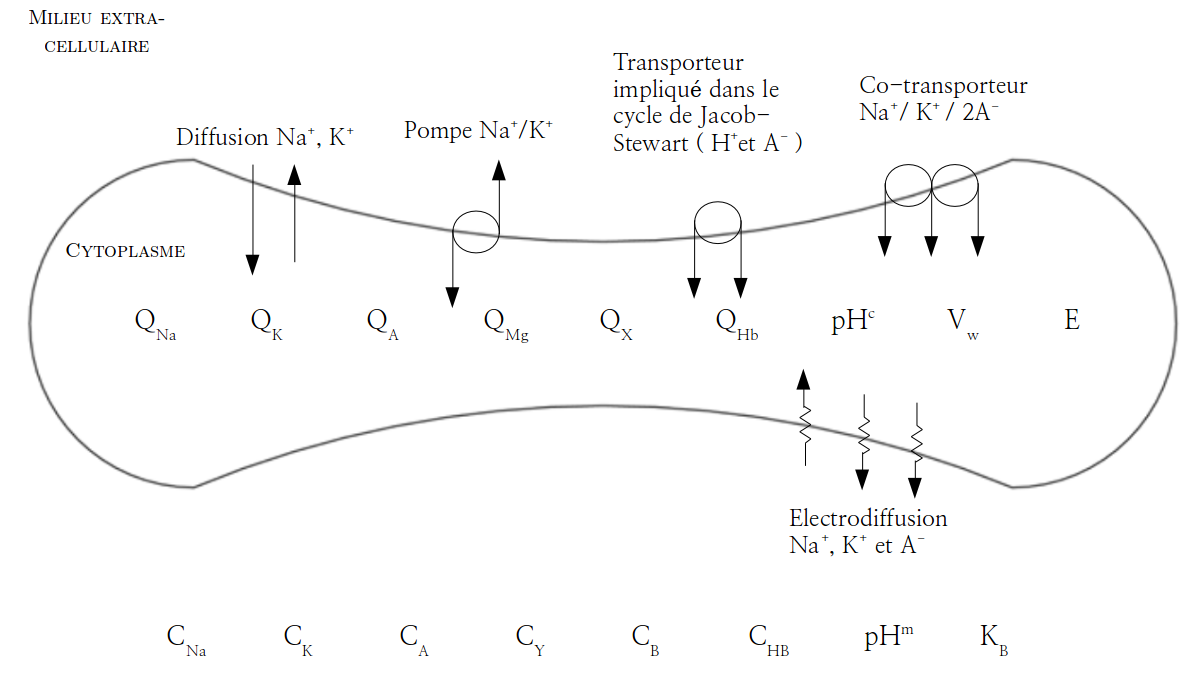
\includegraphics[width=\textwidth]{globule_rouge.png}
\caption{Flux et variables du modèle du globule rouge}
\end{figure} 


\newpage

\tableofcontents              % Table des matières

\newpage

% \part{Titre}                % Commencer une partie...

\section{Modèle et notations}               % Commencer une section, etc.

Afin de caractériser les flux à travers la membrane plasmique du globule rouge, nous considérerons les espèces chimiques suivantes :

\begin{tabular}{p{11cm}cr}
\textbf{Espèces chimiques}                                                   & \textbf{Abréviation} \\
\\
Sodium                                                            & ${Na}$   \\
Potassium                                                         & $K$    \\
Magnesium                                                         & ${Mg}$   \\
Hydrogène                                                          & $H$    \\
Hémoglobine                                                       & ${Hb}$   \\
Anion perméant                                                    & $A$    \\
Anion imperméant intracellulaire considéré comme non protonisable & $X$    \\
Anion monovalent imperméant extracellulaire                       & $Y$    \\
Tampon imperméant extracellulaire                                 & $B$    \\
Forme protonisée du tampon                                        & ${HB}$   \\

\end{tabular}\\
\\


Nous définissons ensuite les variables d'intérêt du système, où $i$ correspond à une des espèces citées plus haut, dans la mesure où la variable s'applique à celle-ci: \\
\\

\begin{tabular}{p{8cm}lr}

\textbf{Variable}                                                      & \textbf{Abréviation}     & \textbf{Unité}      \\
\\
Quantité de l'espèce $i$ dans un litre de solution de cellules compactées \footnotemark[1]  & $Q_i$                    & $mmol.loc^{-1}$     \\
Concentration de l'espèce $i$ dans le milieu extracellulaire               & $C_{i}^{m}$              & $mmol.l^{-1}$       \\
pH intracellulaire                                                     & $pH^c$                                         \\
pH extracellulaire                                                     & $pH^m$                                         \\
Volume de cytoplasme dans un litre de solution de cellules compactées \footnotemark[1]	& $V_w$ 			 & $l.loc^{-1}$      \\
Volume d'hématocrite dans un litre de sang (taux d'hématocrite)             & $Ht$          & $l.l^{-1}$                   \\
Volume de liquide extracellulaire dans un litre de sang                     & $V_s$                    & $l.l^{-1}$        \\
Flux total de l'espèce $i$ (nécessairement perméant)                       & $\Phi_i$                 & $mmol.loc^{-1}.h^{-1}$\\
Flux partiel à travers la pompe Na: K de l'espèce $i$                      & $\Phi_{i}^{P}$           & $mmol.loc^{-1}.h^{-1}$\\
Flux partiel lié à la diffusion de l'espèce $i$                             & $\Phi_{i}^{L}$           & $mmol.loc^{-1}.h^{-1}$\\
Flux partiel lié à l'électrodiffusion de l'espèce $i$                      & $\Phi_{i}^{G}$           & $mmol.loc^{-1}.h^{-1}$\\
Flux partiel à travers le co-transporteur Na: K: 2A de l'espèce $i$         & $\Phi_{i}^{Co}$          & $mmol.loc^{-1}.h^{-1}$\\
Flux partiel à travers le co-transporteur H: A de l'espèce $i$              & $\Phi_{i}^{HA}$          & $mmol.loc^{-1}.h^{-1}$\\
Coefficient osmotique de l'hémoglobine                                 & $f_{Hb}$                                       \\

\end{tabular}\\
\\
\\

\footnotetext[1]{La solution de cellules compactées est une solution composée uniquement d'hématocrite, ne contenant pas de liquide extracellulaire} 



\begin{tabular}{p{8cm}cr}

\textbf{Paramètres}                                             & \textbf{Abréviation}     & \textbf{Unité}      \\
Volume intracellulaire initial                                 & $V_{w}^{\left(0\right)}$                       \\
Perméabilité de l'espèce $i$ lors de la diffusion                  & $P_{i}^{L}$              & $h^{-1}$            \\
Perméabilité de l'espèce $i$ lors de l'électrodiffusion            & $P_{i}^{G}$              & $h^{-1}$            \\
Constante de turnover du co-transport Na: K: 2A (Co)            & $k_{Co}$                                       \\
Constante de turnover du co-transport H: A (HA)                 & $k_{HA}$                                       \\
Valence de l'ion $i$                                             & $z_i$                                          \\
Constante de Faraday                                           & $F$                      & $s.A.mol^{-1}$      \\
Constante des gaz parfaits                                     & $R$                      & $J.mol^{-1}.K^{-1}$ \\
Température absolue                                            & $T$                      & $K$                 \\
pH isoélectrique de l'hémoglobine                              & $pI$                                           \\
Constante de dissociation de la solution tampon B              & $K_B$                    & $mol.l^{-1}$        \\
Coefficients viriaux de l'équation de $f_{Hb}$                 & $b, c$                   &                     \\
Facteur de compensation dans le co-transport Na: K: 2A          & $d$                      &                     \\
Flux saturé de Na à travers la pompe Na: K                   & $\Phi^{max}_{Na}$        & $mmol.loc^{-1}.h^{-1}$ \\

\end{tabular}\\
\\


\section{Équations constitutives}

\subsection{Quelques équations utiles pour la suite}

\subsubsection*{Potentiel de membrane}
\begin{equation}
E=\dfrac{-RT}{F}\,\ln\left(\dfrac{P_{Na}^{G}\,\dfrac{Q_{Na}}{V_w}+P_{K}^{G}\,\dfrac{Q_{K}}{V_w}+P_{A}^{G}\,C_{A}^{m}}{P_{Na}^{G}\,C_{Na}^{m}+P_{K}^{G}\,C_{K}^{m}+P_{A}^{G}\,\dfrac{Q_{A}}{V_w}}\right)
\end{equation}\\

Sous l'hypothèse que la somme des flux électrodiffusifs est nulle :

\begin{equation}
\sum z_i\Phi_{i}^G = 0\label{eq:FLuxG}
\end{equation}

Afin de prendre en compte les variations du potentiel de membrane $E$ du globule rouge, il nous fallait une équation pour le calculer. Nous sommes donc partis de l'hypothèse que la somme des flux liés à l'électrodiffusion pondérés par la valence de l'ion du flux est égale à zéro (équation~\eqref{eq:FLuxG}). On a alors :

\begin{equation}
\Phi_{Na}^G+\Phi_{K}^G-\Phi_{A}^G=0
\end{equation}

On explicite alors les différents flux liés à l'électrodiffusion :

\begin{multline}
-P_{Na}^{G}\,\frac{FE}{RT}\left(\frac{\dfrac{Q_{Na}}{V_w}\,-\,{C_{Na}^{m}\exp{\dfrac{-FE}{RT}}}}{1 - \exp{\dfrac{-FE}{RT}}}\right)-P_{K}^{G}\,\frac{FE}{RT}\left(\dfrac{\dfrac{Q_{K}}{V_w}-{C_{K}^{m}\,\exp{\dfrac{-FE}{RT}}}}{1 - \exp{\dfrac{-FE}{RT}}}\right)\\
-P_{A}^{G}\,\frac{FE}{RT}\left(\dfrac{\dfrac{Q_{A}}{V_w}\,-\,{C_{K}^{m}\exp{\dfrac{+FE}{RT}}}}{1 - \exp{\dfrac{+FE}{RT}}}\right)=0
\end{multline}

On ramène tout au même dénominateur et on simplifie par le facteur commun différent de $0$ :

\begin{multline}
-P_{Na}^{G}\,\frac{FE}{RT}\left(\frac{\dfrac{Q_{Na}}{V_w}\,-\,{C_{Na}^{m}\exp{\dfrac{-FE}{RT}}}}{1 - \exp{\dfrac{-FE}{RT}}}\right)-P_{K}^{G}\,\frac{FE}{RT}\left(\dfrac{\dfrac{Q_{K}}{V_w}-{C_{K}^{m}\,\exp{\dfrac{-FE}{RT}}}}{1 - \exp{\dfrac{-FE}{RT}}}\right)\\
+P_{A}^{G}\,\frac{FE}{RT}\left(\dfrac{\dfrac{Q_{A}}{V_w}\exp{\dfrac{-FE}{RT}}\,-\,C_{A}^{m}}{1 - \exp{\dfrac{-FE}{RT}}}\right)=0
\end{multline}


\begin{equation}
-P_{Na}^{G}\,\dfrac{Q_{Na}}{V_w}-P_{K}^{G}\,\dfrac{Q_{K}}{V_w}-P_{A}^{G}\,C_{A}^{m}+P_{Na}^{G}\,C_{Na}^{m}\exp{\dfrac{-FE}{RT}}+P_{K}^{G}\,C_{K}^{m}\,\exp{\dfrac{-FE}{RT}}+P_{A}^{G}\,\dfrac{Q_{A}}{V_w}\exp{\dfrac{-FE}{RT}}=0
\end{equation}

Enfin, on isole $E$ pour obtenir l'équation finale :

\begin{equation}
\exp{\dfrac{-FE}{RT}}=\dfrac{P_{Na}^{G}\,\dfrac{Q_{Na}}{V_w}+P_{K}^{G}\,\dfrac{Q_{K}}{V_w}+P_{A}^{G}\,C_{A}^{m}}{P_{Na}^{G}\,C_{Na}^{m}+P_{K}^{G}\,C_{K}^{m}+P_{A}^{G}\,\dfrac{Q_{A}}{V_w}}
\end{equation}

\begin{equation*}
E=\dfrac{-RT}{F}\,\ln\left(\dfrac{P_{Na}^{G}\,\dfrac{Q_{Na}}{V_w}+P_{K}^{G}\,\dfrac{Q_{K}}{V_w}+P_{A}^{G}\,C_{A}^{m}}{P_{Na}^{G}\,C_{Na}^{m}+P_{K}^{G}\,C_{K}^{m}+P_{A}^{G}\,\dfrac{Q_{A}}{V_w}}\right)
\end{equation*}

\subsubsection*{Concentration extracellulaire de H (dont on a besoin pour déterminer $\Phi^{HA}$)}
\begin{equation}
{C_{H}^{c,m}=\exp_{10}{\left(-pH^{c,m}\right)}}\Longleftrightarrow{pH^{c,m}=-\log{\left(-C_{H}^{c,m}\right)}}\label{eq:pH}
\end{equation}

\begin{equation}
C_{H}^{m}=K_B\,\dfrac{C_{HB}^m}{C_{B}^m-C_{HB}^m}
\end{equation}

\subsubsection*{Variation de $Ht$}
D'après la publication de Virgilio L.LEW et Robert M.BOOKCHIN : 
\begin{equation}
V_s = 1-Ht \label{eq:Vs}
\end{equation}

et
\begin{equation}
\dfrac{dV_s}{dt} = -\dfrac{dV_w}{dt}Ht \label{eq:dVs}
\end{equation}\\

En dérivant~\eqref{eq:Vs}, on obtient donc que les variations de $Ht$ et $V_s$ sont opposées :
\begin{equation}
\dfrac{dV_s}{dt} = -\dfrac{dHt}{dt}
\end{equation} \\

Sachant cela et en s'appuyant sur l'équation~\eqref{eq:dVs}, on en déduit que :
\begin{equation}
Ht = Ht_0\,\exp{(V_w-V_w^0)} \label{eq:Ht} 
\end{equation}\\

\subsection{Equations liées aux flux}
\subsubsection*{Équations des différents flux}

\begin{equation}
\Phi_{Na}^{P}=-\Phi_{max}^{Na}\left(\frac{\dfrac{Q_{Na}}{V_w}}{\dfrac{Q_{Na}}{V_w} + 0.1\left(1+\dfrac{Q_{K}}{8.3\,V_w}\right)}\right)^3\left(\dfrac{C_{K}^{m}}{C_{K}^{m}+0.1\left(1+\dfrac{C_{Na}^{m}}{18}\right)}\right)^2
\end{equation}

\begin{equation}
\Phi_{K}^{P}=-\frac{\Phi_{Na}^{P}}{1.5}
\end{equation}

\begin{equation}
\Phi_{Na}^{L}=-P_{Na}^{L}\left(\frac{Q_{Na}}{V_w}-C_{Na}^{m}\right)
\end{equation}

\begin{equation}
\Phi_{K}^{L}=-P_{K}^{L}\left(\frac{Q_{K}}{V_w}-C_{K}^{m}\right)
\end{equation}

\subsubsection*{Équations des flux électrodiffusifs}

\begin{equation}
\Phi_{Na}^{G}=-P_{Na}^{G}\,\frac{FE}{RT}\left(\frac{\dfrac{Q_{Na}}{V_w}\,-\,{C_{Na}^{m}\exp{\dfrac{-FE}{RT}}}}{1 - \exp{\dfrac{-FE}{RT}}}\right)
\end{equation}

\begin{equation}
\Phi_{K}^{G}=-P_{K}^{G}\,\frac{FE}{RT}\left(\dfrac{\dfrac{Q_{K}}{V_w}-{C_{K}^{m}\,\exp{\dfrac{-FE}{RT}}}}{1 - \exp{\dfrac{-FE}{RT}}}\right)
\end{equation}

\begin{equation}
\Phi_{A}^{G}=+P_{A}^{G}\,\frac{FE}{RT}\left(\dfrac{\dfrac{Q_{A}}{V_w}\,-\,{C_{K}^{m}\exp{\dfrac{+FE}{RT}}}}{1 - \exp{\dfrac{+FE}{RT}}}\right)
\end{equation}

\subsubsection*{Équations du cotransporteur Na:K:A}

\begin{equation}
\Phi_{A}^{Co}=-k_{Co}\left(\frac{Q_{A}^2\,Q_{Na}\,Q_{K}}{V_w^4}-d\left(C_{A}^{m}\right)^2C_{Na}^{m}C_{K}^{m}\right)
\end{equation}

\begin{equation}
\Phi_{Na}^{Co}=\Phi_{K}^{Co}=\frac{\Phi_{A}^{Co}}{2}
\end{equation}

\subsubsection*{Équation du flux HA}

\begin{equation}
\Phi_{H}^{HA}=\Phi_{A}^{HA}=-k_{HA}( \frac{Q_A\,Q_H}{V_w^2} - C_{A}^{m}\,C_{H}^{m})
\end{equation}\\

\subsection{Système d'équations différentielles}

\begin{empheq}[left=\empheqlbrace]{align}
\frac{dQ_{Na}}{dt}&=\Phi_{Na}=\Phi_{Na}^{P}+\Phi_{Na}^{L}+\Phi_{Na}^{G}+\Phi_{Na}^{Co}\label{eq:dQNadt}\\
\frac{dQ_K}{dt}&=\Phi_{K}=\Phi_{K}^{P}+\Phi_{K}^{L}+\Phi_{K}^{G}+\Phi_{K}^{Co}\label{eq:dQKdt}\\
\frac{dQ_A}{dt}&=\Phi_{A}=\Phi_{A}^{G}+\Phi_{A}^{HA}+\Phi_{A}^{Co}\label{eq:dQAdt}\\
\frac{dQ_H}{dt}&=\Phi_{H}=\Phi_{H}^{HA}\label{eq:dQHdt}\\
\frac{dV_w}{dt}&= \frac{\dfrac{dQ_{Na}}{dt}+\dfrac{dQ_K}{dt}+\dfrac{dQ_A}{dt}}{C_{Na}^{m}+C_{K}^{m}+C_{A}^{m}+C_{B}^{m}+C_{Y}^{m}}\label{eq:dVwdt}\\
\frac{dC_{Na}^m}{dt}&=\frac{Ht}{1 - Ht}\left(C_{Na}^m\,\dfrac{dV_w}{dt}-\frac{dQ_{Na}}{dt}\right)\label{eq:dCmNadt}\\
\frac{dC_{K}^m}{dt}&=\frac{Ht}{1 - Ht}\left(C_{K}^m\,\dfrac{dV_w}{dt}-\frac{dQ_{K}}{dt}\right)\label{eq:dCmKdt}\\
\frac{dC_{A}^m}{dt}&=\frac{Ht}{1 - Ht}\left(C_{A}^m\,\dfrac{dV_w}{dt}-\frac{dQ_{A}}{dt}\right)\label{eq:dCmAdt}\\
\frac{dC_{HB}^m}{dt}&=\frac{Ht}{1 - Ht}\left(C_{HB}^m\,\dfrac{dV_w}{dt}-\frac{dQ_{H}}{dt}\right)\label{eq:dCmHBdt}\\
\frac{dC_{B}^m}{dt}&=\frac{Ht}{1 - Ht}\,C_{B}^m\,\dfrac{dV_w}{dt}\label{eq:dCmBadt}\\
\frac{dC_{Y}^m}{dt}&=\frac{Ht}{1 - Ht}\,C_{Y}^m\,\dfrac{dV_w}{dt}\label{eq:dCmYdt}\\
\end{empheq}

\subsection{Expliquation des formules du système d'équations différentielles}

Pour les variations des quantités intracellulaires des ions (équations~\eqref{eq:dQNadt} à ~\eqref{eq:dQHdt}) nous avons utilisé les formules de la publication de Virgilio L.LEW et Robert M.BOOKCHIN. Pour les variations des concentrations extracellulaires des ions (équations~\eqref{eq:dCmNadt} à ~\eqref{eq:dCmYdt}) nous avons utilisé leur formule :\\
\\
$C_i^{m(t)}=C_i^{m(t-\Delta{t})}\,\left(1 + \dfrac{Ht}{1 - Ht}\,\dfrac{dV_w}{dt}\right) - \dfrac{Ht}{1 - Ht}\,\dfrac{dQ_{i}}{dt}$ ; \\
\\
où $C_i^{m(t)}$ correspond à la concentration extracellulaire de l'ion i à l'instant t et $\Delta{t}$ à une durée infiniment petite. On peut alors écrire :\\
\\
$C_i^{m(t)} - C_i^{m(t-\Delta{t})} = \dfrac{dC_{i}^m}{dt}$\\
\\
Puis en développant dans l'expression de la publication, on obtient :\\
\\
$\dfrac{dC_{i}^m}{dt}=\dfrac{Ht}{1 - Ht}\left(C_{i}^m\,\dfrac{dV_w}{dt}-\dfrac{dQ_{i}}{dt}\right)$
\\

Afin de  d'obtenir un système d'équations différentielles résoluble par \textit{odeint} (bibliothèque \textit{scipy.integrate}), nous avons exprimé la variation du volume intracellulaire indépendamment des variations des concentrations extracellulaires~\eqref{eq:dVwdt}. Pour cela nous avons d'abord réexprimé $V_w$ grâce à l'équation de l'isotonicité et dérivé celle-ci :\\

\begin{equation}
f_{Hb}\,Q_{Hb}+Q_{Na}+Q_K+Q_A+Q_{Mg}+Q_X=V_w\left(C_{Na}^m +C_{K}^m +C_{A}^m +C_{B}^m +C_{Y}^m\right)\label{eq:Volume}
\end{equation}

\begin{equation}
V_{w} = \dfrac{f_{Hb}Q_{Hb}+\sum Q_{i}}{\sum C_{i}^{m}}
\end{equation}

avec
\begin{equation}
\sum Q_{i} = Q_{Na}+Q_{K}+Q_{A}+Q_{Mg}+Q_{X} 
\end{equation}

et 
\begin{equation}
\sum C_{i}^m =C_{Na}^m +C_{K}^m +C_{A}^m +C_{B}^m +C_{Y}^m  
\end{equation}\\

La formule de variation extracellulaire du volume est donc :

\begin{equation}
\dfrac{dV_w}{dt}=\dfrac{\left(\dfrac{dQ_{Na}}{dt}+\dfrac{dQ_K}{dt}+\dfrac{dQ_A}{dt}\right)\left(\sum C_{i}^m\right)-\left(f_{Hb}\,Q_{Hb}+\sum Q_{i}\right)\left(\sum \dfrac{dC_{i}^m}{dt}\right)}{\left(\sum C_{i}^m\right)^2}
\end{equation}

en notant :

\begin{equation}
\sum \dfrac{dQ_i}{dt}=\dfrac{dQ_{Na}}{dt}+\dfrac{dQ_K}{dt}+\dfrac{dQ_A}{dt}
\end{equation}\\

On obtient alors :

\begin{equation}
\dfrac{dV_w}{dt}=\dfrac{\left(\sum \dfrac{dQ_i}{dt}\right)\left(\sum C_{i}^m\right)-\left(f_{Hb}\,Q_{Hb}+\sum Q_{i}\right)\left(\dfrac{Ht}{1-Ht}\left(\dfrac{dV_w}{dt}\,\sum C_{i}^m\,-\sum \dfrac{dQ_i}{dt}\right)\right)}{\left(\sum C_{i}^m\right)^2}
\end{equation}

\begin{multline}
\dfrac{dV_w}{dt}\,\left(\left(\sum C_{i}^m\right)^2+\dfrac{Ht}{1-Ht}\left(f_{Hb}\,Q_{Hb}+\sum Q_{i}\right)\left(\sum \dfrac{dC_{i}^m}{dt}\right)\right)\\
=\left(\sum \dfrac{dQ_i}{dt}\right)\,\left(\sum C_{i}^m\right)+\dfrac{Ht}{1-Ht}\left(f_{Hb}\,Q_{Hb}+\sum Q_{i}\right)\left(\sum \dfrac{dQ_i}{dt}\right)
\end{multline}

\begin{equation}
\dfrac{dV_w}{dt}=\dfrac{\left(\sum \dfrac{dQ_i}{dt}\right)\,\left(\sum C_{i}^m\right)+\dfrac{Ht}{1-Ht}\left(f_{Hb}\,Q_{Hb}+\sum Q_{i}\right)\left(\sum \dfrac{dQ_i}{dt}\right)}{\left(\sum C_{i}^m\right)^2+\dfrac{Ht}{1-Ht}\left(f_{Hb}\,Q_{Hb}+\sum Q_{i}\right)\left(\sum \dfrac{dC_{i}^m}{dt}\right)}
\end{equation}

\begin{equation}
\dfrac{dV_w}{dt}=\dfrac{\left(\sum \dfrac{dQ_i}{dt}\right)\,\left(\sum C_{i}^m+\dfrac{Ht}{1-Ht}\left(f_{Hb}\,Q_{Hb}+\sum Q_{i}\right)\right)}{\left(\sum C_{i}^m\right)\left(\sum C_{i}^m+\dfrac{Ht}{1-Ht}\left(f_{Hb}\,Q_{Hb}+\sum Q_{i}\right)\right)}
\end{equation}

On a finalement :

\begin{equation*}
\dfrac{dV_w}{dt}=\dfrac{\sum \dfrac{dQ_i}{dt}}{\sum C_{i}^m}
\end{equation*}\\


\section{Implémentation}   

Nous avons ensuite implémenté notre système d'équations différentielles en Python. Nous nous sommes servis de Python 3.4.2 pour l'écriture du code et son exécution. Pour résoudre notre système, nous avons utilisé le solveur \textit{odeint} provenant de la bibliothèque \textit{scipy.integrate}. Ce solveur résoud un système d'équations différentielles utilisant LSODA. LSODA (Livermore Solver for Ordinary Differential Equations) permet de résoudre des systèmes de la forme $\dfrac{dy}{dt}=f\left(t,y\right)$, en utilisant une Jacobienne dense ou à bande lorsque le problème est rigide, mais change automatiquement entre une méthode rigide (Backward differentiation formula) et non-rigide (Adams).
Toutes les simulations ont été effectuées sous Ubuntu 16.04 et sous Windows 10, dans l'interpréteur Python \textit{Ipython3}.
   



\section{Application à un cas concret}

Afin de tester notre modèle, nous avons reproduit un des cas présenté dans la publication de Virgilio L.LEW et Robert M.BOOKCHIN ("Effect of a large and sudden increase in the cell K permeability in low-K media", p.69). Les conditions initiales sont les suivantes :\\


\begin{tabular}{p{5cm}lr}
\textbf{Paramètres}                                                   & \textbf{Valeur} \\
\\
$\Phi^{max}_{Na}$ & $8.99$ $mmol.loc^{-1}.h^{-1}$    \\
$d$ & $1.05$   \\
$f_{Hb}$ & $2.78$    \\
$Q_{Hb}$ & $5$ $mmol.loc^{-1}$   \\
$Q_{X}$ & $19.2$ $mmol.loc^{-1}$     \\
$K_B$ & $10^{-4.55}$ $mmol.loc^{-1}$   \\
$P^L_{Na}$ & $0.0020$ $h^{-1}$   \\
$P^L_{K}$ & $0.0013$	 $h^{-1}$   \\
$P^G_{Na}$ & $0.0151$ $h^{-1}$   \\
$P^G_{K}$ & $0.0138 .10^4$ $h^{-1}$   \\
$k_{Co}$ & $10^{-6}$  \\
$k_{HA}$ & $10^{9}$  \\


\end{tabular}\\
\\
\\

\begin{tabular}{p{5cm}lr}
\textbf{Variables à l'état initial}                                                   & \textbf{Valeur} \\
\\
$Q_{Na}$ & $7$ $mmol.loc^{-1}$   \\
$Q_{K}$  & $98$ $mmol.loc^{-1}$     \\
$Q_{A}$ & $66.5$ $mmol.loc^{-1}$ \\
$Q_{H}$ & $700 . 10^{-7.26}$ $mmol.loc^{-1}$    \\
$V_w$ & $0.7$   \\
$C^m_{Na}$ & $140$ $mmol.l^{-1}$     \\
$C^m_K$  & $5$ $mmol.l^{-1}$   \\
$C^m_A$   & $131$ $mmol.l^{-1}$    \\
$C^m_{HB}$  & $5.86$ $mmol.l^{-1}$      \\
$C^m_{B}$  & $10$ $mmol.l^{-1}$      \\
$C^m_{Y}$  & $10$ $mmol.l^{-1}$     \\
$Ht$ & $0.1$   \\

\end{tabular}\\
\\

\textit{NB : Ht est une variable mais elle n'intervient pas dans le système d'équations différentielles, car sa valeur peut être calculée directement à l'aide de celle de $V_w$.}\\
\\

En choisissant un intervalle de temps d'une heure et en faisant varier $P_{A}^{G}$ entre 0.2 et 200 $h^{-1}$, nous obtenons les résultats suivants :

\begin{figure}[H]
\centering 
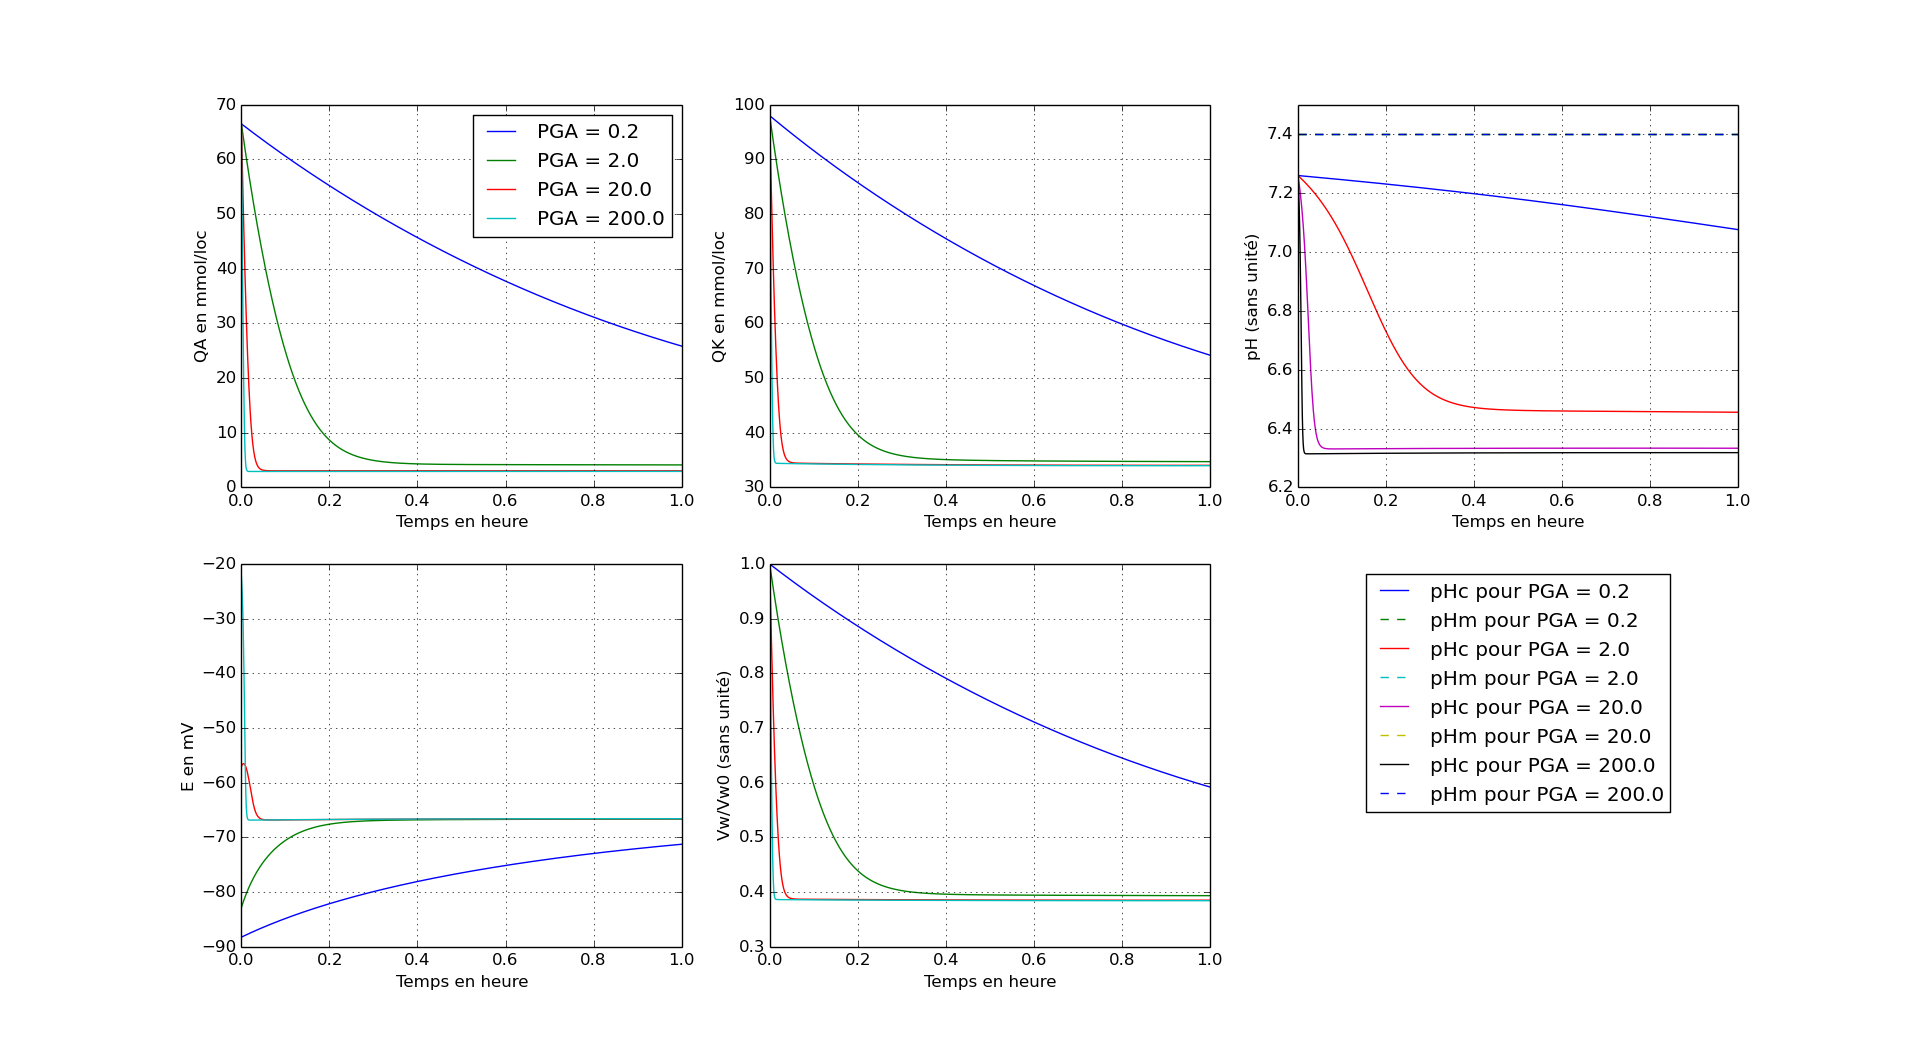
\includegraphics[width=1.1\textwidth]{original_hum.png}
\caption{Variation de $Q_{A}$, $Q_{K}$, $pH^{c}$, $pH^{m}$, $E$ et $V_{w}$ en fonction du temps.}
\label{original}
\end{figure} 

Ces courbes sont très similaires à celles obtenues dans la publication, néanmoins on remarque que quelques valeurs diffèrent légèrement. D'abord la valeur seuil de $\frac{V_w}{V_w^{(0)}}$ devrait se situer aux alentours de 0.63, ensuite la valeur initiale de $E$ est légèrement trop haute pour le cas $P_{A}^{G} = 0.2\,h^{-1}$ : elle devrait se situer à environ -82 mV. Enfin la valeur seuil de $pH^c$ est trop faible ( elle est de 6.3, contre 6.9 dans la publication). Les tendances générales sont donc plutôt bonnes, si on ne tient pas compte du $pH^m$.\\

Le $pH^m$ est la seule variable à ne pas du tout suivre la tendance décrite dans la publication : en se référant à notre modèle, $pH^m$ varie de manière pratiquement négligeable (il apparaît constant sur le graphique, à l'échelle de la variation de $pH^m$), alors qu'il semble être le parfait symétrique vertical de $pH^c$ d'après Virgilio L.LEW et Robert M.BOOKCHIN. Afin de résoudre ce problème, nous avons mis au point différentes versions de notre programme, correspondant chacune à une hypothèse de base.


\section{Différentes versions du code}     

\subsection{Avec et sans solution tampon dans le milieu extracellulaire} 

Plusieurs arguments semblent être en faveur d'un $pH^m$ variant peu. Tout d'abord la solution extracellulaire est définie comme une solution tampon, c'est à dire qu'elle a pour rôle de stabiliser le $pH^m$. Cette solution tampon est matérialisée dans notre modèle par l'espèce chimique $B$ (forme non protonisée) et $HB$ (forme protonisée du tampon). Elle atténue les variations de $H^+$ en se liant ou non avec celui-ci suivant les conditions.\\

Un deuxième argument est que dans notre cas, $Ht$ est fixé au départ à une valeur de 0.1. Cela signifie que le volume extracellulaire est neuf fois plus important que le volume intracellulaire, donc une petite variation de la quantité d'ions hydrogène aura neuf fois plus d'impact en terme de variation de concentration, dans le compartiment intracellulaire que extracellulaire. Cette tendance devrait pouvoir se lire dans le pH, qui devrait varier plus faiblement dans le milieu extracellulaire.\\

Afin de vérifier cette seconde hypothèse, nous avons réécrit le modèle sans tenir compte de la solution tampon. Dans un soucis de clarté, nous avons aussi fixé $P_{A}^{G}$ à $2\,h^{-1}$.\\

Le second modèle ne considérant pas la solution tampon, une hypothèse légitime consistait à définir la quantité totale d'ions $H^+$ comme une constante. \\

\begin{equation}
Q_{tot H} \,= \,C^m_H V_s + Q_H Ht \,=\, C^{m(0)}_H V_s^{(0)} + Q_H^{(0)} Ht^{(0)}
\end{equation} \\

L'expression de $C^m_H$ devient donc :

\begin{equation}
C^m_H = \frac{Q_{tot H}-Q_H Ht}{V_s} 
\end{equation} 

Et celle de $pH^m$, d'après l'équation~\eqref{eq:pH} :

\begin{equation}
pH^m = -\log\left(\frac{Q_{tot H}-Q_H Ht}{V_s}\right)
\end{equation} \\

A l'aide de ces deux versions, nous avons obtenus les graphiques suivant : 

\begin{figure}[H]
\centering 
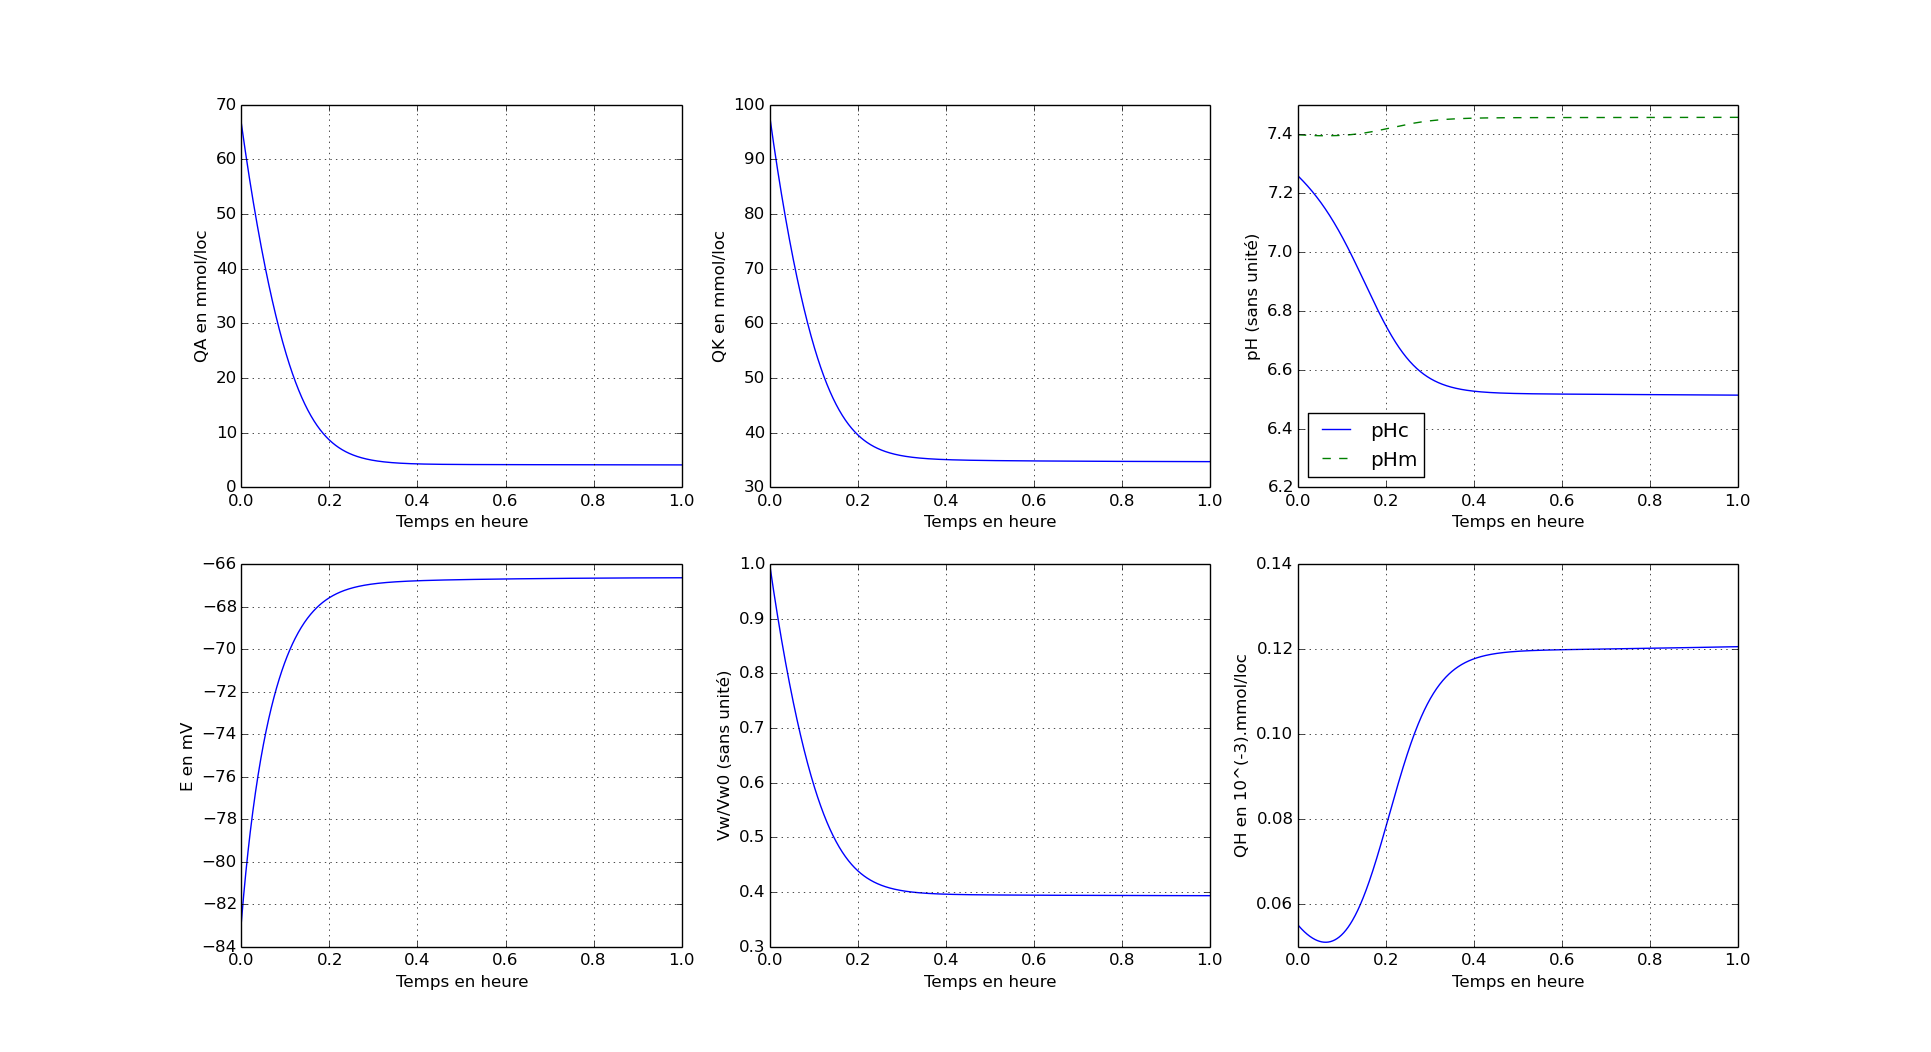
\includegraphics[width=1.1\textwidth]{sans_sol_tampon.png}
\caption{Version modifiée du code omettant la solution tampon.}
\end{figure} 

\begin{figure}[H]
\centering 
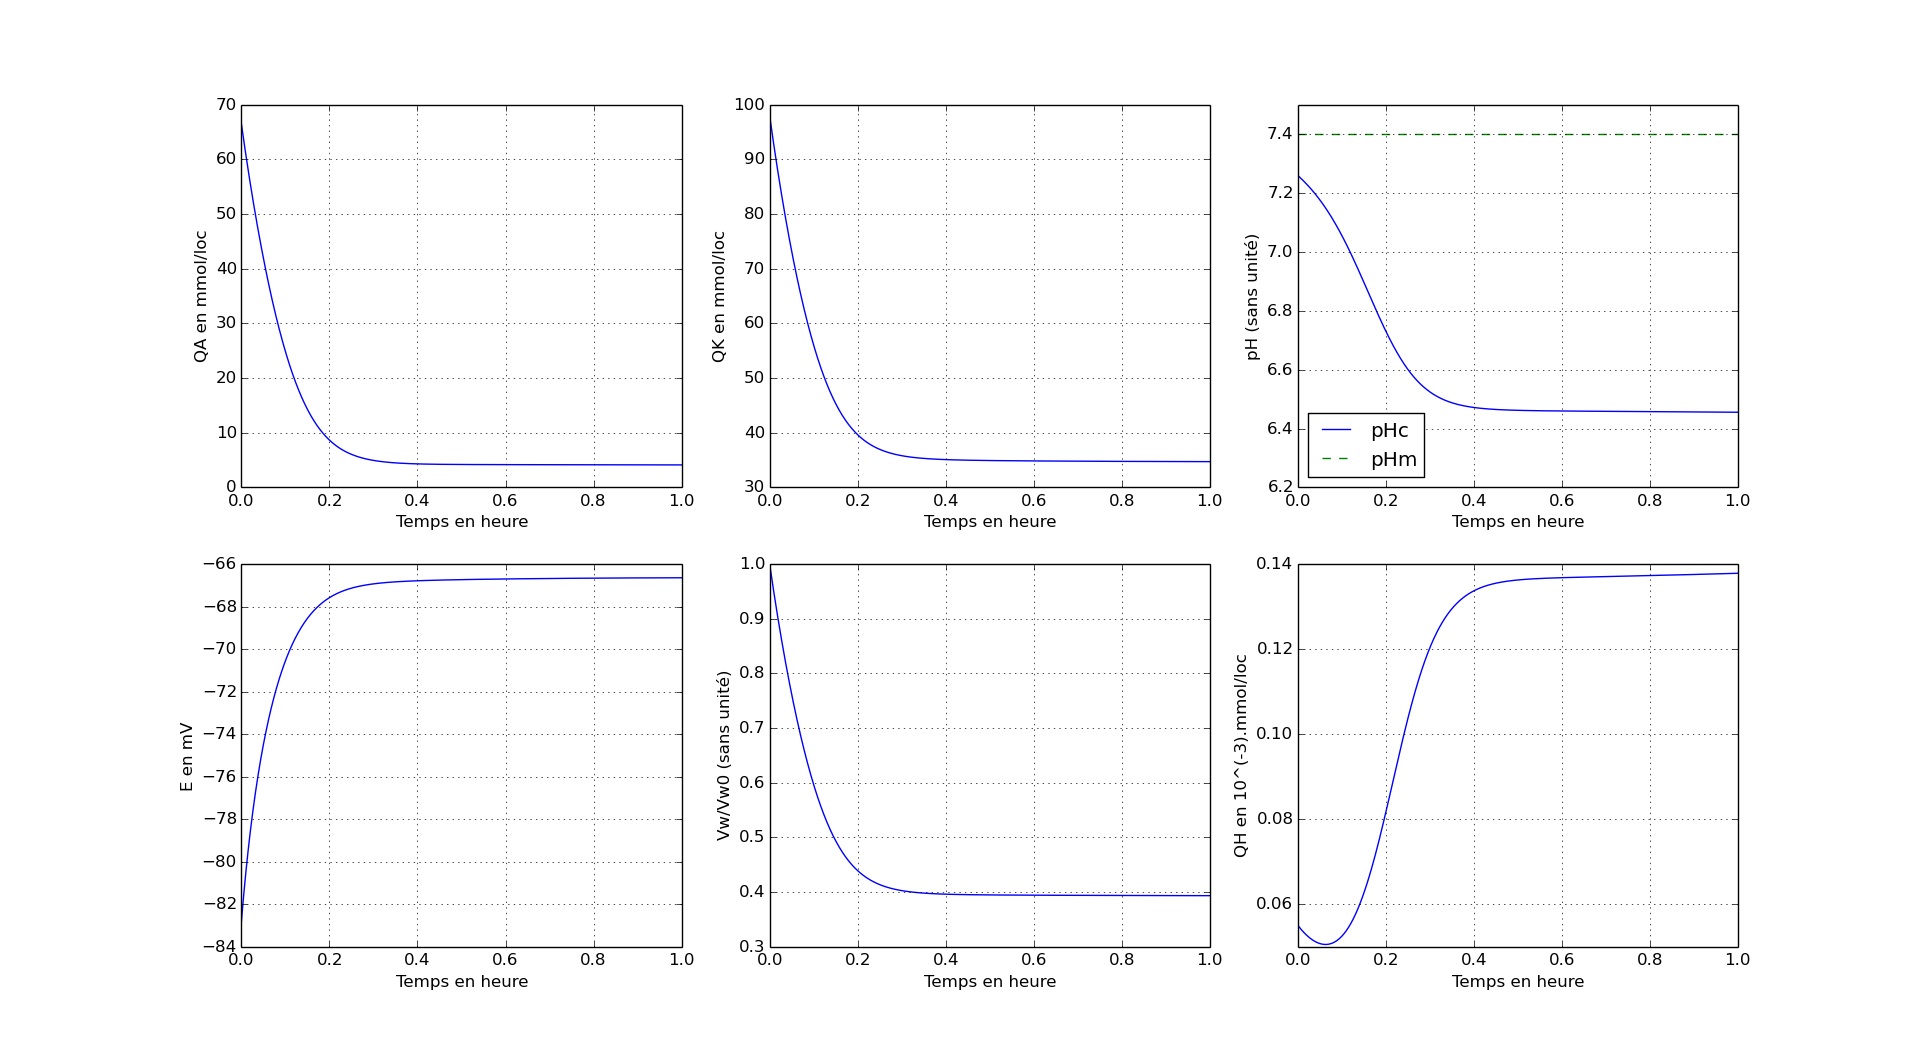
\includegraphics[width=1.1\textwidth]{avec_sol_tampon.png}
\caption{Version du code initiale, considérant la solution tampon.}
\end{figure} 


Comme nous l'attendions, dans la version du code modifiée nous retrouvons une variation du $pH^m$ de plus faible amplitude que celle de $pH^c$ et de sens contraire à celui-ci. Cette petite variation sera encore plus atténuée en présence de solution tampon, il semble donc normal qu'elle soit pratiquement invisible dans la version du code initiale.\\

Les autres variables gardent un comportement inchangé, mis à part la quantité intracellulaire de $H^+$. En effet, en supprimant la solution tampon nous modifions l'équilibre des ions hydrogènes. Les ions $H^+$ qui ont ici tendance à rentrer dans le globule rouge, formeront un flux d'autant plus important que la concentration extracellulaire $C_H^m$ est importante. On observe que la solution tampon agit dans notre cas afin d'éviter que le milieu extracellaire ne devienne trop basique, elle a donc tendance à libérer des ions $H^+$ et de ce fait, augmenter la concentration d'ions hydrogènes dans la solution extracellulaire. Par conséquent, le flux d'ions $H^+$ est alors plus important, et la variation de $Q_H$ plus forte en présence de la solution tampon.\\

L'ensemble de nos résultats semblant en adéquation avec les réalités biologiques, nous pouvons supposer que la version originale de notre modèle reflète réellement l'équilibre atteint au sein du globule rouge dans les conditions que nous avons définies.\\

\subsection{En considérant $f_{Hb}$ variable} 

Dans un premier temps afin de simplifier la mise en équation du modèle, nous avons considéré $f_{Hb}$ constant ($f_{Hb}$ est le coefficient osmotique de l'hémoglobine). En réalité, cette quantité varie et est définie dans la publication de Virgilio L.LEW et Robert M.BOOKCHIN de la façon suivante:

\begin{equation}
f_{Hb}=1+b\,\frac{Q_{Hb}}{V_w }+{c}\left(\frac{Q_{Hb}}{V_w }\right)^2
\end{equation}


Dans une troisième version du code, nous avons remplacé $f_{Hb}$ par sa vraie expression. La valeur des différentes constantes est détaillée dans le tableau ci-dessous, et $PGA$ a encore une fois été fixé à $2\,h^{-1}$. Les résultats obtenus sont présentés dans la figure ci-contre.\\ 
\\

\begin{tabular}{p{3cm}lr}
\textbf{Paramètres}                                                   & \textbf{Valeur} \\
$b$ & $0.0645$    \\
$c$ & $0.0258$   \\
\end{tabular}

\begin{figure}[H]
\centering 
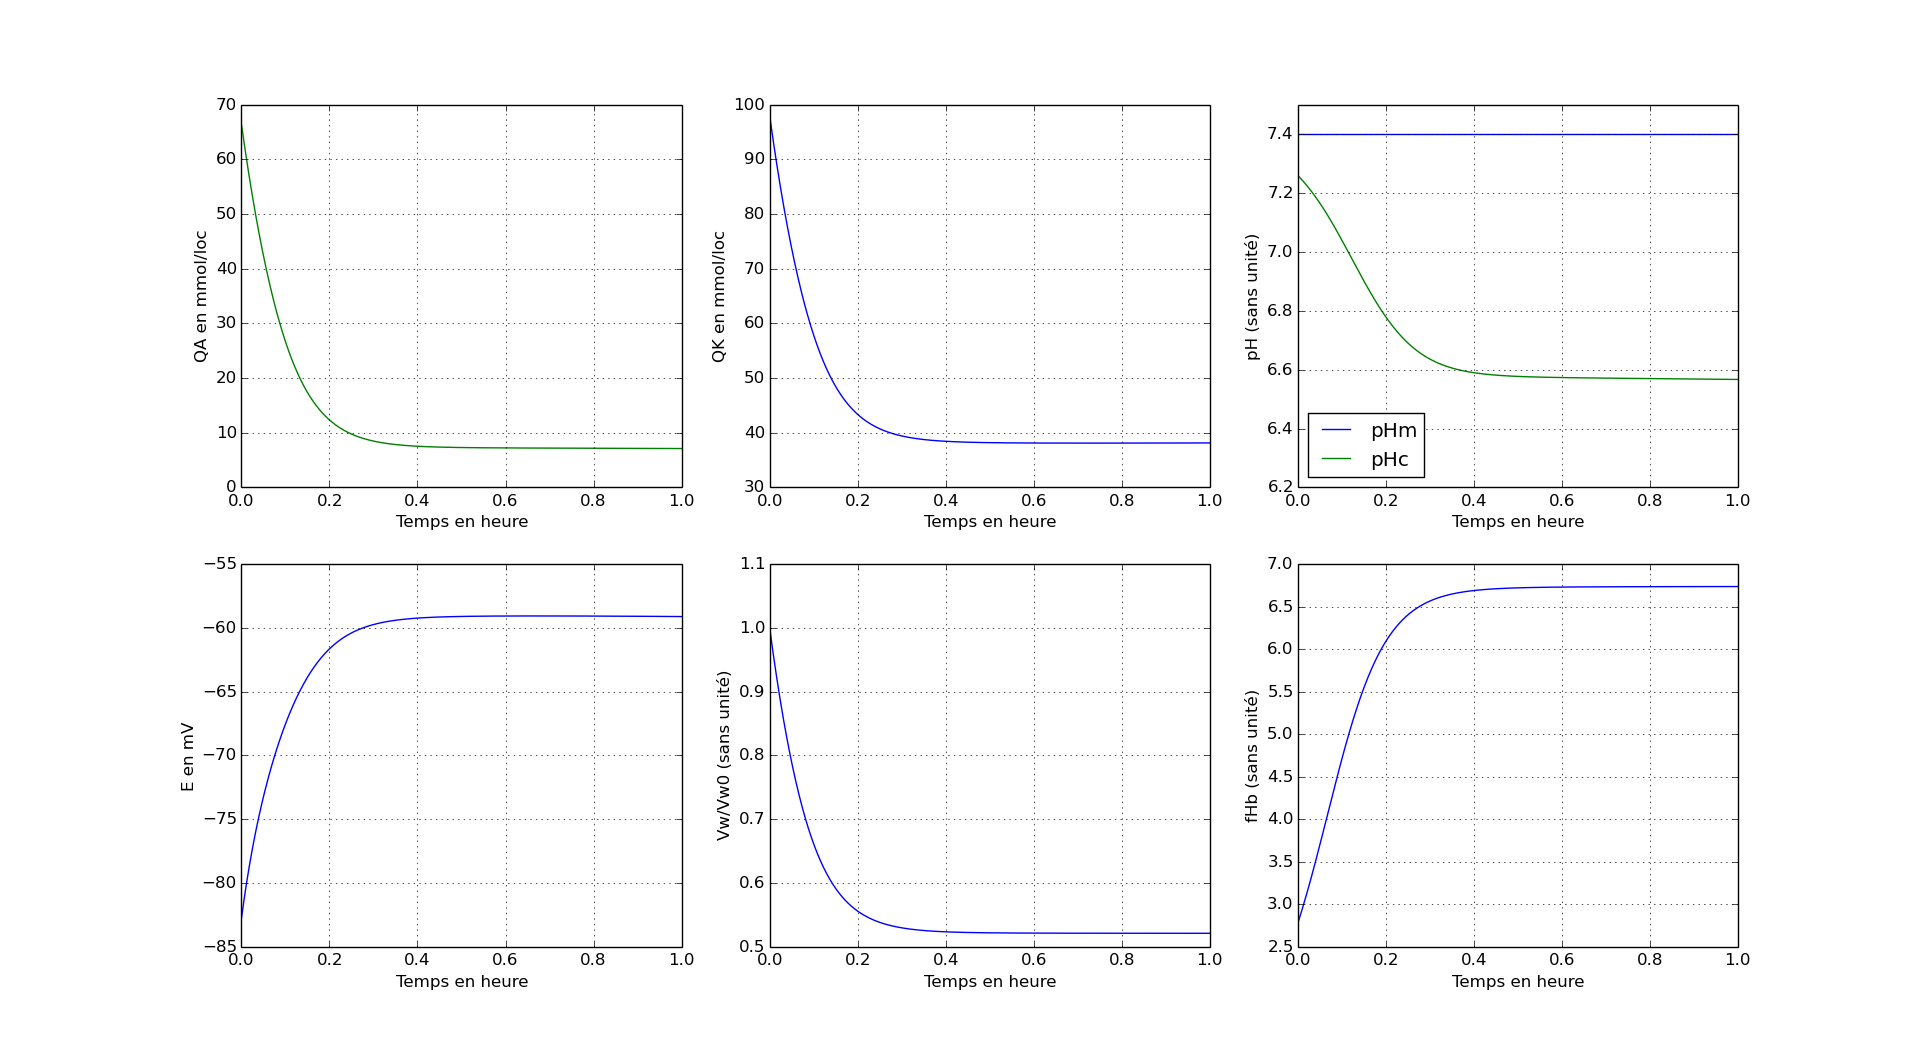
\includegraphics[width=1.1\textwidth]{avec_fhb.png}
\caption{Version modifiée du code, avec $f_{Hb}$ variable.}
\end{figure} 

En rajoutant les variations de $f_{Hb}$, on remarque que les erreurs observées sur certaines des quantités physico-chimiques de la figure~\ref{original} sont atténuées, même si elles restent présentes (valeurs de $\frac{V_w}{V_w^{(0)}}$ et $pH^c$). \\

La valeur de $f_{Hb}$ est elle aussi légèrement plus différente (6.7 contre 7.5 dans la publication).\\


\section{Conclusion} 

L'implémentation ayant donné des résultats semblables à ceux de la publication, il est maintenant intéressant de les confronter aux données expérimentales obtenues par les chercheurs, afin d'affiner certains paramètres ou fonctions. Le but est qu'à terme, le programme puisse servir en laboratoire afin de prédire les résultats d'expériences réalisées dans des conditions données. Le présent rapport a également fait l'objet d'une soutenance pendant laquelle des biologistes ont pu poser des questions et apporter leur opinion sur ce programme. \\

Le code est disponible sur la plateforme \textit{GitHub}, à l'adresse ci-dessous :

\url{https://github.com/SaiOne/Red_Blood_Cell}\\

Les références complètes de l'article sont :

Lew,V.L., Bookchin, R.M. 1986. Volume, pH, and Ion-Content Regulation in Human Red Cells : Analysis of Transient Behavior with  an Integrate Model. \textit{J. Membrane Biol}. \textbf{92}:57-74.\\
 

% \paragraph{Titre}           % Toutes petites sections (le nom \paragraph
                              % n'est pas très bien choisi)

% \subparagraph{Titre}        % La dernière

% \appendix                   % Commençons les annexes

% \section{Titre}             % Annexe A

% \section{Titre}             % Annexe B

% \listoffigures              % Table des figures

% \listoftables               % Liste des tableaux

\end{document}
